\documentclass[12pt]{article}
\usepackage{helvet}
\usepackage{graphicx}
\usepackage{geometry}
\geometry{
    a4paper,
    top = 2cm,
    left = 2cm,
    right = 2cm,
    bottom = 3cm
}
\usepackage[utf8]{inputenc}
\usepackage[spanish,mexico]{babel} % Renombra en automático los elementos a español
\addto\captionsspanish{
  \renewcommand{\figurename}{Imagen}
  \renewcommand{\tablename}{Tabla}
}
\usepackage{float}  % Etiqueta 'H' (mayus) en figuras (imágenes)
\usepackage{array}  % Padding en tablas
\usepackage{tabularx}
\usepackage{url}    % Etiqueta url en .bib
\usepackage{booktabs}   % Manejo de caudros (tablas)
\usepackage[T1]{fontenc}    % Codificación de fuentes
\usepackage[autostyle, spanish=mexican]{csquotes}       % Paquete para comillas tipográficas
\usepackage{comment}    % Comentar bloques de líneas mediante begin-end
\usepackage{multicol}   % Para poner contenido a doble columna
\usepackage{enumitem}   % Para utilizar [noitemsep, topsep=0pt] en itemize
\usepackage{amsmath}
\usepackage{mathabx} % Para testar en math mode
\usepackage{comment}
\usepackage{longtable}
\usepackage[hidelinks]{hyperref}
\usepackage{caption}
\usepackage[
  backend=biber,
  style=apa,
  sorting=nyt
]{biblatex}
\DeclareLanguageMapping{spanish}{spanish-apa}
\renewcommand{\familydefault}{\sfdefault}
\newenvironment{localsubgroup}
  {$\left\{\tabular{l}}
  {\endtabular\right.$}


\addbibresource{bibliography/t08.bib}

\begin{comment}
INDICACIONES DEL PROFESOR:
Investigar los siguientes conceptos de seguridad

Conceptos de seguridad informática.

¿Qué es Ciberseguridad y sus conceptos básicos?

Define los siguientes conceptos: amenaza, vulnerabilidad, ataque e intruso.

¿Qué es malware y sus diferentes variedades?

¿Qué herramientas existen para proteger los sistemas?

¿Cuáles son algunas recomendaciones para protección de la información?

El máximo de hojas es 25.

RESTRICCIÓN DE EXTENSIÓN:
Rango: 18 a 25 páginas (máximo riguroso de 25 hojas). Objetivo de desarrollo: 22 a 24 páginas.

ÍNDICE APROBADO:
1. Fundamentos de seguridad informática [2.5 págs.]
   1.1. Objetivos y principios de la seguridad
   1.2. Tríada de confidencialidad, integridad y disponibilidad
   1.3. Modelos formales de seguridad y control de acceso
2. Definición y alcance de la ciberseguridad [2.5 págs.]
   2.1. Ciberespacio y perímetro de protección
   2.2. Diferencias entre ciberseguridad y seguridad de la información
   2.3. Superficies y vectores de exposición
3. Amenazas, vulnerabilidades, ataques e intrusos [3.5 págs.]
   3.1. Interrelación conceptual y modelo de riesgo
   3.2. Clasificación y naturaleza de las amenazas
   3.3. Vulnerabilidades en software y sistemas operativos
   3.4. Mecanismos y fases de ejecución de ataques
   3.5. Tipología de intrusos y modelos de intrusión
4. Software malicioso y sus variedades [4.0 págs.]
   4.1. Definición y taxonomía estructural del malware
   4.2. Malware parasitario e infeccioso: virus y bombas lógicas
   4.3. Malware autorreplicable en red: gusanos
   4.4. Software de infiltración y control: troyanos, puertas traseras y rootkits
   4.5. Malware de extorsión y espionaje: ransomware, spyware y botnets
5. Herramientas para la protección de sistemas [4.5 págs.]
   5.1. Cortafuegos y filtrado de tráfico en capas
   5.2. Sistemas de detección y prevención de intrusos (IDS/IPS)
   5.3. Motores antimalware y detección en puntos terminales (EDR)
   5.4. Mecanismos de aislamiento y endurecimiento del núcleo
   5.5. Cifrado de almacenamiento y comunicaciones del sistema
   5.6. Herramientas de auditoría y análisis de vulnerabilidades
6. Recomendaciones para la protección de la información [3.0 págs.]
   6.1. Principio de mínimo privilegio y defensa en profundidad
   6.2. Endurecimiento de configuración del sistema operativo
   6.3. Gestión de parches y mitigación continua de fallos
   6.4. Esquemas de respaldo y recuperación ante desastres
   6.5. Autenticación multifactor y control de identidades
   6.6. Registro de eventos, monitoreo y respuesta a incidentes
7. Conclusiones personales [2.0 págs.]
   (Estructura monolítica continua: 2 cuartillas)
Referencias bibliográficas [1.0 pág.]
Total estimado acumulado: 22 a 24 páginas (máx. 25).
\end{comment}

\begin{document}
\pagenumbering{roman}

\begin{titlepage}
  \thispagestyle{empty}
  \newgeometry{left = 1cm, right = 1cm, top = 1cm, bottom = 2cm}

  \noindent
  \begin{minipage}[c]{3.5cm}
    
\includegraphics[width=3.5cm]{media/titlepage/Escudo-UNAM.pdf}
  \end{minipage}\hfill
  \begin{minipage}[c][3.5cm][c]{\dimexpr\textwidth-7cm\relax}
    \centering
    {\large\textbf{Universidad Nacional Autónoma de México}\\[0.6em] 
    \Large\textbf{Facultad de Ingeniería}\\[0.6em]
    \large Sistemas Operativos}
  \end{minipage}\hfill
  \begin{minipage}[c]{3.5cm}
    \raggedleft
    
\includegraphics[width=3.5cm]{media/titlepage/FI.png}
  \end{minipage}
\centering\huge
  \vfill
    Grupo 1 \\
    Ing. Angel Isidro Mercado
  \vfill
    \textbf{Tarea 8. Herramientas de trabajo}
  \vfill\large
    320304435 - Cabrera Rojas Oscar
  \vfill

  \noindent\footnotesize \hfill Ciudad Universitaria, CDMX a 19 de noviembre del 2026
\end{titlepage}
\restoregeometry

\tableofcontents

\newpage
\pagenumbering{arabic}
\setcounter{page}{1}

\section{Fundamentos de seguridad informática}\label{sec:fundamentosSeguridadInformatica}

El diseño y operación de los sistemas informáticos contemporáneos descansan sobre la capacidad del sistema operativo (SO) para gestionar recursos compartidos, aislar tareas computacionales y garantizar la convivencia armónica entre múltiples usuarios y procesos. En entornos multiprogramados y conectados en red, la seguridad informática deja de ser una característica secundaria para transformarse en un requisito estructural del núcleo (\textit{kernel}). Sin mecanismos rigurosos de protección y control, la concurrencia y la compartición de recursos degeneran inevitablemente en corrupción de memoria, fuga de información confidencial y colapso de la disponibilidad del sistema frente a eventos accidentales o intenciones maliciosas.

\subsection{Objetivos y principios de la seguridad}\label{subsec:objetivosPrincipiosSeguridad}

En la teoría de sistemas operativos es indispensable formular una distinción precisa entre los conceptos de protección y seguridad. La protección comprende los mecanismos internos del sistema diseñados para controlar y restringir el acceso de los programas, procesos y usuarios hacia los recursos físicos y lógicos administrados por el computador, tales como regiones de memoria principal, descriptores de archivos, dispositivos de entrada/salida y ciclos de la unidad central de procesamiento (CPU) \parencite[\S 14.1, p.\ 483]{silberschatz2006fundamentos}. Por su parte, la seguridad representa una cualidad global y omnicomprensiva: constituye la medida de confianza en que el sistema, sus datos y sus canales de comunicación se mantendrán libres de accesos no autorizados, modificaciones fraudulentas y destrucciones intencionadas, abarcando tanto los mecanismos internos del núcleo como las salvaguardas externas de autenticación, criptografía y administración física \parencite[\S 15.1, p.\ 509]{silberschatz2006fundamentos}.

Uno de los pilares de la ingeniería de seguridad reside en la estricta separación conceptual entre políticas y mecanismos \parencite[\S 14.1, p.\ 484]{silberschatz2006fundamentos}. Las políticas definen qué acciones y qué tipos de acceso están permitidos o prohibidos para cada clase de usuario y recurso en una organización determinada; los mecanismos constituyen las estructuras y procedimientos concretos del hardware y del software mediante los cuales se imponen dichas políticas en tiempo de ejecución. Mientras que las políticas de una entidad cambian con frecuencia debido a normativas legales o reorganizaciones operativas, los mecanismos del núcleo deben permanecer estables, flexibles y desacoplados, permitiendo implementar esquemas de autorización diversos sin requerir la reescritura del sistema operativo \parencite[\S 19.4.2, p.\ 888]{deitel2004operating}.

La construcción de sistemas confiables se rige por principios de diseño fundamentales formulados formalmente por Saltzer y Schroeder. Entre ellos, el \textbf{principio de mínimo privilegio} (\textit{least privilege}) establece que a cada sujeto (usuario, proceso o hilo) se le deben conceder exclusivamente los privilegios indispensables para llevar a cabo su tarea durante el menor tiempo posible \parencite[\S 14.2, p.\ 484]{silberschatz2006fundamentos}, acotando el radio de impacto ante fallos de programación o intrusiones maliciosas. Este postulado se complementa con la \textbf{economía de mecanismos} (\textit{economy of mechanism}), que prescribe una arquitectura del núcleo concisa para facilitar su verificación formal, y con la \textbf{mediación completa} (\textit{complete mediation}), que exige que cada intento de acceso a cualquier recurso protegido sea interceptado y validado en tiempo de ejecución, impidiendo el uso de autorizaciones previas cacheadas erróneamente.

Asimismo, el criterio de \textbf{valores por omisión seguros} (\textit{fail-safe defaults}) determina que la denegación de acceso debe ser el estado predeterminado ante cualquier solicitud carente de permiso explícito. El principio de \textbf{diseño abierto} (\textit{open design}) sostiene que la seguridad no debe depender del secreto de los algoritmos o de la arquitectura interna del sistema, sino de la custodia adecuada de claves criptográficas y credenciales. Finalmente, la \textbf{separación de privilegios} (\textit{separation of privilege}) demanda que las operaciones críticas dependan del cumplimiento simultáneo de múltiples condiciones o de la concurrencia de dos o más entidades de control independientes.

\subsection{Tríada de confidencialidad, integridad y disponibilidad}\label{subsec:triadaCia}

La evaluación formal del estado de seguridad de un sistema informático se fundamenta en tres dimensiones canónicas interdependientes, agrupadas bajo la denominación de tríada CIA (\textit{Confidentiality, Integrity, Availability}):

La \textbf{confidencialidad} garantiza que los activos de información y los recursos del sistema no sean divulgados ni resulten accesibles a sujetos o procesos no autorizados \parencite[\S 2, p.\ 72]{rfc4949}. A nivel del sistema operativo, la confidencialidad se implementa mediante la segmentación y paginación de memoria virtual, la cual aísla los espacios de direccionamiento de los procesos, el control riguroso de permisos en el sistema de archivos y el empleo de algoritmos criptográficos para salvaguardar datos almacenados y transmisiones de red \parencite[\S 15.1, p.\ 509]{silberschatz2006fundamentos}.

La \textbf{integridad} asegura que los datos y los componentes lógicos del sistema permanezcan exactos, consistentes y libres de modificaciones no autorizadas o corrupciones maliciosas \parencite[\S 2, p.\ 146]{rfc4949}. La literatura técnica distingue entre la integridad de los datos, orientada a impedir escrituras o borrados arbitrarios sobre la información almacenada, y la integridad del sistema, que garantiza que el núcleo y los servicios del sistema operativo ejecuten sus algoritmos conforme a la especificación prevista, sin desvíos provocados por manipulación de memoria o inyección de código \parencite[\S 2.1, p.\ 6]{nistSp800_12}.

La \textbf{disponibilidad} establece la certidumbre de que los recursos computacionales y los servicios del sistema se encuentren operativos y accesibles oportunamente para los usuarios autorizados cuando estos los requieran \parencite[\S 2, p.\ 28]{rfc4949}. En el núcleo, este precepto demanda esquemas de planificación de CPU resistentes a la inanición (\textit{starvation}), gestión robusta del bloqueo mutuo (\textit{deadlock}) y mecanismos de cuotas y limitación de tasas para repeler ataques de denegación de servicio (DoS, \textit{denial-of-service}) que busquen agotar la memoria, los descriptores de archivos o el ancho de banda \parencite[\S 15.1, p.\ 510]{silberschatz2006fundamentos}.

Junto a la tríada clásica, los estándares contemporáneos integran tres dimensiones complementarias imprescindibles para la trazabilidad y el rigor normativo: la \textbf{autenticidad}, que valida la identidad genuina de usuarios, procesos y mensajes; el \textbf{no repudio}, que impide que un emisor o receptor niegue formalmente haber efectuado o recibido una transacción digital determinada; y la \textbf{rendición de cuentas} (\textit{accountability}), que garantiza la capacidad técnica de auditar cada evento y atribuir unívocamente la autoría de cada operación ejecutada dentro del sistema mediante registros de bitácora protegidos contra manipulación \parencite[\S 2.1, p.\ 6]{nistSp800_12}.

\subsection{Modelos formales de seguridad y control de acceso}\label{subsec:modelosFormalesControlAcceso}

Para imponer las directivas de seguridad en la interacción cotidiana entre programas y datos, los sistemas operativos recurren a abstracciones matemáticas de control de acceso. El modelo clásico formulado por Lampson define una matriz de acceso en la que las filas representan a los sujetos $S$ (entidades activas con capacidad de ejecutar acciones, típicamente procesos que operan en nombre de usuarios), las columnas corresponden a los objetos $O$ (entidades pasivas protegidas, como archivos, regiones de memoria o dispositivos) y cada celda $A[s, o]$ contiene el conjunto de derechos de acceso $R$ asignados al sujeto $s$ sobre el objeto $o$ \parencite[\S 14.4, p.\ 489]{silberschatz2006fundamentos}, \parencite[\S 15.3, p.\ 670]{stallings2018operating}.

Dado que la matriz de acceso es intrínsecamente dispersa debido a la gran cantidad de combinaciones posibles entre sujetos y objetos del sistema, los núcleos de los sistemas operativos la implementan mediante dos estructuras de descomposición complementarias, detalladas en la Img.~\ref{fig:estructurasControlAcceso}: la descomposición por columnas o \textbf{listas de control de acceso} (ACL, \textit{access control lists}), donde cada objeto almacena una lista explícita de identificadores de usuario o grupos junto con los privilegios concedidos sobre él (como POSIX ACL en Unix/Linux o DACL en NTFS de Windows) \parencite[\S 15.3, p.\ 671]{stallings2018operating}; y la descomposición por filas o \textbf{listas de capacidades} (\textit{capabilities}), donde cada sujeto posee una colección de fichas o credenciales infalsificables resguardadas por el núcleo que describen los objetos accesibles y las operaciones permitidas \parencite[\S 14.5, p.\ 493]{silberschatz2006fundamentos}.

\begin{figure}[htbp]
    \centering
    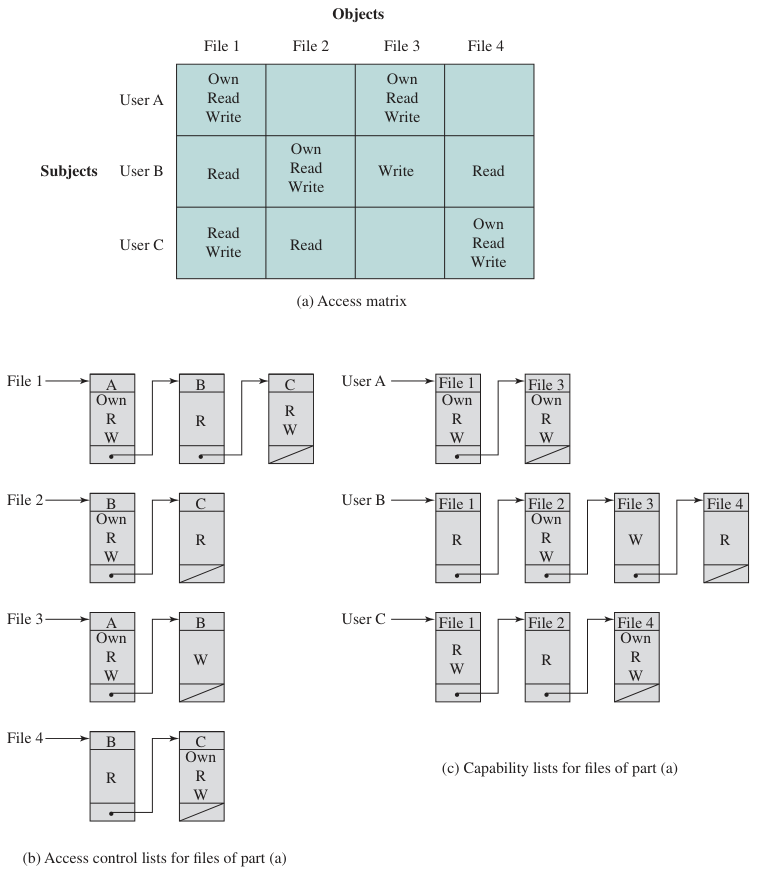
\includegraphics[width=\textwidth]{media/t08/estructurasControlAcceso.png}
    \caption{Estructuras de control de acceso: matriz general, listas de control de acceso y listas de capacidades \parencite[\S 15.3, p.\ 671]{stallings2018operating}.}
    \label{fig:estructurasControlAcceso}
\end{figure}

A partir de estas estructuras, la literatura formal categoriza las políticas de control de acceso en cuatro esquemas operativos primarios \parencite[\S 15.3, p.\ 672]{stallings2018operating}, \parencite[\S 19.4.2, p.\ 888]{deitel2004operating}. El \textbf{control de acceso discrecional} (DAC, \textit{discretionary access control}) permite que el propietario de un objeto posea la potestad de definir y delegar los permisos sobre su recurso, constituyendo el esquema imperante en permisos Unix tradicionales. En contraste, el \textbf{control de acceso obligatorio} (MAC, \textit{mandatory access control}) impone directivas centralizadas e inmutables por los usuarios, comparando etiquetas de sensibilidad en los objetos frente a niveles de acreditación (\textit{clearances}) de los sujetos. Por su parte, el \textbf{control de acceso basado en roles} (RBAC, \textit{role-based access control}) asigna permisos a perfiles organizacionales y vincula dinámicamente a los usuarios a dichos roles, mientras que el \textbf{control de acceso basado en atributos} (ABAC, \textit{attribute-based access control}) evalúa dinámicamente propiedades del sujeto, del recurso y del contexto ambiental.

En sistemas multinivel de alta criticidad, las políticas de seguridad se formalizan mediante modelos matemáticos de flujo de información. El \textbf{modelo de Bell-LaPadula} se orienta a la preservación estricta de la confidencialidad a través de dos axiomas cardinales: la \textit{propiedad de seguridad simple} (\enquote{no leer hacia arriba} o \textit{no read up}), que veta el acceso a datos de mayor clasificación; y la \textit{propiedad estrella} (\textit{$\star$-property}, \enquote{no escribir hacia abajo} o \textit{no write down}), que prohíbe transferir información hacia objetos de menor nivel, neutralizando la fuga de secretos. En contraparte, el \textbf{modelo de Biba} es el dual estricto enfocado en la integridad: prescribe la \textit{propiedad de integridad simple} (\enquote{no leer hacia abajo} o \textit{no read down}) y la \textit{propiedad estrella de integridad} (\enquote{no escribir hacia arriba} o \textit{no write up}), impidiendo que sujetos confiables consuman datos espurios o corrompan capas superiores. Finalmente, el \textbf{modelo de Clark-Wilson} adapta la integridad al terreno comercial mediante el uso exclusivo de procedimientos de transformación bien formados (\textit{well-formed transactions}) y la separación obligatoria de deberes. La Tabla~\ref{tab:comparativaModelosControlAcceso} sintetiza los fundamentos de estos modelos y su correspondencia práctica en el sistema operativo.

\begin{table}[htbp]
\centering
\footnotesize
\renewcommand{\arraystretch}{1.1}
\renewcommand{\tabularxcolumn}[1]{m{#1}}
\setlength{\emergencystretch}{1.5em}
\caption{Comparativa técnica de políticas y modelos formales de control de acceso.}
\label{tab:comparativaModelosControlAcceso}
\begin{tabularx}{\textwidth}{>{\centering\arraybackslash}m{2.4cm} X X}
\toprule
\textbf{Modelo / Política} & \textbf{Criterio de decisión y propiedades formales} & \textbf{Mecanismo e impacto en el sistema operativo} \\
\midrule
\textbf{DAC} & Discrecional según el dueño; verificación de identidad y pertenencia a grupos. & Permisos clásicos en inodos Unix (\textit{user, group, other}) y listas DACL en sistemas NTFS. \\
\addlinespace
\textbf{MAC} & Comparación forzosa entre etiquetas de seguridad y acreditaciones del sujeto; imposición central. & Módulos LSM (\textit{Linux Security Modules}) en el núcleo como SELinux y Smack bajo reglas TE. \\
\addlinespace
\textbf{RBAC} & Autorizaciones asignadas a perfiles funcionales o roles; mapeo desacoplado de usuarios. & Módulos PAM (\textit{Pluggable Authentication Modules}) y esquemas de elevación acotada con \textit{sudo}. \\
\addlinespace
\textbf{Bell-LaPadula} & Confidencialidad multinivel; axiomas \enquote{no leer hacia arriba} y \enquote{no escribir hacia abajo} ($\star$-\textit{property}). & Políticas MLS (\textit{Multi-Level Security}) en núcleos certificados para defensa y custodia de secretos. \\
\addlinespace
\textbf{Biba} & Integridad estricta; axiomas \enquote{no leer hacia abajo} y \enquote{no escribir hacia arriba}. & Mecanismos de protección del núcleo contra controladores no verificados e integridad de procesos críticos. \\
\addlinespace
\textbf{Clark-Wilson} & Integridad comercial mediante transacciones bien formadas y separación obligatoria de deberes. & Subsistemas de bases de datos con control transaccional ACID y verificación de firmas en binarios del sistema. \\
\bottomrule
\end{tabularx}
\end{table}

\section{Definición y alcance de la ciberseguridad}\label{sec:definicionAlcanceCiberseguridad}

La convergencia global de infraestructuras computacionales, redes de transporte de datos y servicios distribuidos ha reconfigurado sustancialmente el entorno operativo de los sistemas. En este contexto interconectado, la seguridad ya no puede concebirse exclusivamente como un conjunto de mecanismos de aislamiento residentes en un computador aislado. La naturaleza omnipresente de las comunicaciones digitales introduce un espacio operacional complejo y continuo denominado ciberespacio, el cual impone nuevos desafíos de defensa y exige una delimitación conceptual rigurosa frente a disciplinas afines.

\subsection{Ciberespacio y perímetro de protección}\label{subsec:ciberespacioPerimetroProteccion}

La norma internacional ISO/IEC 27032 define formalmente el ciberespacio como el entorno complejo resultante de la interacción dinámica entre personas, software y servicios en Internet mediante dispositivos tecnológicos y redes interconectadas que carecen de una manifestación física tangible \parencite[\S 4.14, p.\ 3]{iso27032}. Lejos de ser un mero medio de transporte de paquetes, el ciberespacio constituye un dominio operacional transversal en el que convergen la infraestructura física de conmutación y enrutamiento, la capa lógica del sistema operativo y protocolos de red, la capa semántica de la información procesada y el plano de interacción social y económica de los usuarios.

Históricamente, la protección de los sistemas se estructuraba en torno al concepto de perímetro de red (\textit{network perimeter}). Bajo este paradigma tradicional, la arquitectura de seguridad establecía una frontera física y lógica neta custodiada por cortafuegos perimetrales, concentradores de red privada virtual (VPN, \textit{virtual private network}) y zonas desmilitarizadas (DMZ, \textit{demilitarized zone}), asumiendo que todo tráfico interno proveniente de la red corporativa era confiable, mientras que el exterior era inherentemente hostil \parencite[\S 19.6.1, p.\ 939]{deitel2004operating}.

La transformación contemporánea de las infraestructuras ---impulsada por la dispersión del trabajo remoto, el cómputo en la nube, los servicios distribuidos y los dispositivos móviles--- ha provocado la disolución irrevocable del perímetro defensivo clásico. En los entornos modernos, las amenazas no provienen únicamente de fronteras externas, sino que habitan potencialmente dentro de la propia red local debido a compromisos de credenciales o dispositivos infectados. En consecuencia, la ingeniería de sistemas operativos y de red ha transitado hacia el modelo de arquitectura de confianza cero (\textit{Zero Trust Architecture}). Este enfoque descarta la noción de confianza implícita por ubicación topológica y exige que cada sujeto, proceso y paquete de red sea autenticado, autorizado y cifrado de forma continua antes de permitir cualquier interacción con los recursos protegidos del sistema operativo \parencite[\S 15.5, p.\ 681]{stallings2018operating}.

\subsection{Diferencias entre ciberseguridad y seguridad de la información}\label{subsec:diferenciasCiberseguridadSeguridadInformacion}

En el ámbito técnico y profesional suele incurrirse en la confusión conceptual entre seguridad de la información, seguridad informática y ciberseguridad. Aunque las tres disciplinas comparten la preservación de la tríada de confidencialidad, integridad y disponibilidad, difieren notablemente en su alcance operativo, el universo de activos bajo su custodia y las metodologías de mitigación empleadas \parencite[\S 2.1, p.\ 5]{nistSp800_12}, \parencite[\S 3.1, p.\ 2]{itutX1205}:

La \textbf{seguridad de la información} (\textit{information security}) constituye la disciplina integradora de mayor jerarquía. Su propósito cardinal reside en salvaguardar la información en cualquiera de sus formas de existencia (documentos impresos en papel, conocimiento verbal, datos digitales o registros archivísticos) contra el acceso no autorizado, la divulgación, la alteración o la destrucción, abarcando controles administrativos, legales, físicos y organizacionales.

Por su parte, la \textbf{seguridad informática} (\textit{computer security}) se concentra en los sistemas computacionales en sí mismos. Su foco operativo abarca el hardware, el firmware, los componentes del sistema operativo y el software aplicativo local, procurando que los procesadores, la memoria principal y los dispositivos de almacenamiento ejecuten exclusivamente instrucciones legítimas y preserven la integridad del núcleo frente a fallos lógicos o abusos locales de privilegios \parencite[\S 15.1, p.\ 509]{silberschatz2006fundamentos}.

En contraste, la \textbf{ciberseguridad} (\textit{cybersecurity}) se orienta específicamente hacia los riesgos, agresiones y eventos adversos que se originan, transitan o explotan a través del ciberespacio y las redes interconectadas \parencite[\S 1, p.\ 1]{iso27032}. La ciberseguridad trasciende la mera protección de los datos estáticos: ampara la estabilidad y resiliencia de los servicios en línea, protege la integridad de las infraestructuras críticas (sistemas de control industrial SCADA, redes eléctricas, plataformas financieras) y resguarda a los usuarios contra el fraude digital y la manipulación social a gran escala. La Tabla~\ref{tab:comparativaDisciplinasSeguridad} sintetiza las diferencias estructurales entre estas tres dimensiones de la seguridad.

\begin{table}[htbp]
\centering
\footnotesize
\renewcommand{\arraystretch}{1.1}
\renewcommand{\tabularxcolumn}[1]{m{#1}}
\setlength{\emergencystretch}{1.5em}
\caption{Comparativa técnica entre seguridad de la información, seguridad informática y ciberseguridad.}
\label{tab:comparativaDisciplinasSeguridad}
\begin{tabularx}{\textwidth}{>{\centering\arraybackslash}m{2.5cm} X X}
\toprule
\textbf{Disciplina} & \textbf{Alcance operativo y activos protegidos} & \textbf{Medio de amenaza y foco de mitigación} \\
\midrule
\textbf{Seguridad de la información} & Omnicomprensivo; protege todo activo de información de la organización (física, digital, verbal o archivística). & Accesos indebidos, divulgación no autorizada y destrucción física; gobernanza organizacional y marcos ISO/IEC 27001. \\
\addlinespace
\textbf{Seguridad informática} & Sistemas de cómputo individuales y locales; hardware, memoria, núcleo del sistema operativo y software de base. & Fallos de aislamiento de procesos, errores lógicos locales, escalada indebida de privilegios y control de acceso DAC/MAC. \\
\addlinespace
\textbf{Ciberseguridad} & Activos digitales, servicios en red, infraestructuras críticas y usuarios interconectados a través del ciberespacio. & Agresiones originadas en redes públicas, vectores distribuidos de denegación de servicio (DDoS), malware en red y cibercrimen. \\
\bottomrule
\end{tabularx}
\end{table}

\subsection{Superficies y vectores de exposición}\label{subsec:superficiesVectoresExposicion}

El análisis de la susceptibilidad de un sistema frente a intrusiones externas requiere examinar la relación entre su superficie de ataque y los vectores de exposición que permiten alcanzarla. La \textbf{superficie de ataque} (\textit{attack surface}) se define formalmente como la suma acumulativa de todos los puntos de entrada, interfaces de comunicación y canales accesibles a través de los cuales un agente hostil no autorizado puede intentar introducir datos, extraer información sensible o forzar la ejecución de código no confiable dentro del sistema.

Desde la perspectiva de la arquitectura de sistemas, la superficie de ataque se descompone en tres planos fundamentales:
\begin{itemize}[noitemsep, topsep=2pt]
    \item \textbf{Superficie de red:} Constituida por la totalidad de puertos abiertos en protocolos de transporte (TCP y UDP), servicios de escucha (demonios SSH, servidores web, llamadas a procedimiento remoto RPC), protocolos de enrutamiento y puertos físicos o interfaces de red inalámbricas expuestas \parencite[\S 15.5, p.\ 682]{stallings2018operating}. Cada socket abierto representa un canal potencial de explotación si el proceso que lo atiende contiene defectos de validación.
    \item \textbf{Superficie de software y sistema operativo:} Abarca las interfaces de llamadas al sistema (\textit{system calls}) expuestas por el núcleo a procesos de usuario no privilegiados, los mecanismos de comunicación interproceso (IPC), los analizadores de sintaxis (\textit{parsers}) encargados de procesar formatos de archivos complejos (como certificados digitales, imágenes o cabeceras de red) y los demonios con privilegios de administrador (\textit{root} o \textit{SYSTEM}) que reciben entradas del exterior \parencite[\S 15.1, p.\ 658]{stallings2018operating}.
    \item \textbf{Superficie humana y organizacional:} Comprende a los usuarios, operadores y administradores del sistema, quienes interactúan directamente con los activos mediante credenciales de autenticación y pueden ser inducidos a error mediante técnicas de ingeniería social o incurrir en negligencias de configuración.
\end{itemize}

Por su parte, un \textbf{vector de ataque} (\textit{attack vector}) representa la vía, técnica o mecanismo específico empleado por un atacante para aprovechar una debilidad presente en la superficie de ataque y entregar una carga maliciosa (\textit{payload}) o vulnerar las políticas del sistema \parencite[\S 15.1, p.\ 511]{silberschatz2006fundamentos}. Entre los vectores de mayor relevancia en sistemas conectados figuran la inyección remota de paquetes malformados hacia servicios de red para inducir desbordamientos de búfer (\textit{buffer overflow}), la falsificación de identidad mediante suplantación de remitente (\textit{phishing}) para sustraer credenciales y el envenenamiento de repositorios en cadenas de suministro de software.

La defensa robusta del sistema exige una política estricta de reducción de la superficie de ataque mediante el endurecimiento (\textit{hardening}) del sistema operativo \parencite[\S 15.5, p.\ 683]{stallings2018operating}. Este proceso implica desinstalar o inhabilitar todos los servicios, protocolos y paquetes innecesarios, aplicar la segmentación estricta de interfaces mediante cortafuegos locales de filtrado de paquetes, restringir las capacidades de llamadas al sistema permitidas a procesos no confiables mediante mecanismos de filtrado (como \textit{seccomp} en Linux) y someter las aplicaciones expuestas a confinamiento obligatorio bajo dominios de seguridad reforzados.

\section{Amenazas, vulnerabilidades, ataques e intrusos}\label{sec:amenazasVulnerabilidadesAtaquesIntrusos}

El análisis riguroso de la seguridad informática requiere descomponer los incidentes de seguridad en sus componentes causales constitutivos. En la literatura técnica y en los estándares internacionales, los términos amenaza, vulnerabilidad, ataque e intruso no son sinónimos intercambiables, sino conceptos estrictamente delimitados que interactúan de forma secuencial y determinista en la degradación de un sistema de cómputo.

\subsection{Interrelación conceptual y modelo de riesgo}\label{subsec:interrelacionConceptualRiesgo}

La dinámica operativa de la seguridad se articula en torno a la protección de los activos (\textit{assets}), entendidos como los recursos de hardware, software, datos y servicios que poseen valor intrínseco para una organización y cuya afectación compromete sus objetivos operativos. Sobre estos activos, los conceptos clave se interrelacionan en una cadena causal definida:
\begin{enumerate}[noitemsep, topsep=2pt]
    \item Una \textbf{vulnerabilidad} representa una debilidad, fallo o defecto latente presente en el activo o en su entorno operativo.
    \item Una \textbf{amenaza} constituye la fuerza o agente potencial con la capacidad de aprovechar dicha debilidad para causar un perjuicio.
    \item Un \textbf{intruso} o agente de amenaza es el actor específico (humano o automatizado) que orquesta la agresión.
    \item Un \textbf{ataque} es la materialización deliberada de la amenaza mediante la ejecución de acciones concretas sobre la vulnerabilidad identificada.
\end{enumerate}

El resultado final de esta interacción genera un impacto adverso sobre el activo. En la ingeniería de sistemas, este fenómeno se formaliza mediante el concepto de riesgo, el cual cuantifica la probabilidad de que una amenaza determinada explote con éxito una vulnerabilidad concreta, ponderada por la magnitud del daño que dicha explotación inflige al sistema \parencite[\S 2, p.\ 14]{nistSp800_30}:
\begin{equation}\label{eq:modeloRiesgo}
\text{Riesgo} = \mathcal{P}(\text{Amenaza} \mid \text{Vulnerabilidad}) \times \text{Impacto}
\end{equation}

Esta formulación evidencia que la mera presencia de una vulnerabilidad no genera un riesgo inmediato si no existe un vector de amenaza capaz de alcanzarla; análogamente, una amenaza masiva resulta inofensiva sobre un componente debidamente blindado y carente de fallos de diseño o configuración.

\subsection{Clasificación y naturaleza de las amenazas}\label{subsec:clasificacionNaturalezaAmenazas}

El estándar RFC 4949 define una \textbf{amenaza} (\textit{threat}) como la circunstancia, evento o potencialidad de que una violación de seguridad ocurra a través de la explotación deliberada o accidental de una vulnerabilidad \parencite[\S 2, p.\ 298]{rfc4949}. Las amenazas se categorizan estructuralmente según su comportamiento operativo y su punto de origen:

En primer término, la literatura distingue entre amenazas pasivas y activas \parencite[\S 15.1, p.\ 509]{silberschatz2006fundamentos}:
\begin{itemize}[noitemsep, topsep=2pt]
    \item \textbf{Amenazas pasivas:} Tienen como finalidad exclusiva la interceptación de información y el monitoreo de transmisiones sin alterar el estado del sistema ni perturbar los datos. Se manifiestan típicamente mediante la captura de paquetes en interfaces promiscuas (\textit{sniffing}) o el análisis de tráfico (\textit{traffic analysis}) para deducir patrones de comunicación, identidades y volúmenes de intercambio. Debido a que no dejan huellas de alteración directa en registros o archivos, su detección es extraordinariamente compleja, por lo que su mitigación se basa primordialmente en la prevención mediante cifrado simétrico y asimétrico robusto.
    \item \textbf{Amenazas activas:} Implican la alteración intencionada de los recursos del sistema, la inyección de flujos de datos espurios o la degradación de la operatividad del computador. Se subdividen en: suplantación de identidad o mascarada (\textit{masquerade}), donde un actor finge ser una entidad autorizada; repetición fraudulenta (\textit{replay attacks}), donde un mensaje legítimo capturado previamente es retransmitido para forzar una operación no autorizada; modificación de mensajes en tránsito; y la provocación deliberada de denegación de servicio \parencite[\S 15.1, p.\ 510]{silberschatz2006fundamentos}.
\end{itemize}

En segundo término, según la posición del agente respecto a los límites de confianza, se clasifican en amenazas internas (\textit{insiders}) y externas (\textit{outsiders}). Las amenazas internas provienen de empleados, operadores o procesos legítimos que disponen de acceso autenticado y credenciales válidas en el sistema operativo, lo que les permite abusar de sus privilegios eludiendo cortafuegos perimetrales. Las amenazas externas se originan fuera de la infraestructura de la entidad y requieren vulnerar los controles de acceso iniciales para obtener un punto de apoyo en la red.

\subsection{Vulnerabilidades en software y sistemas operativos}\label{subsec:vulnerabilidadesSoftwareSo}

Una \textbf{vulnerabilidad} (\textit{vulnerability}) es un defecto, debilidad o fallo en el diseño conceptual, la codificación, la configuración o la administración de un componente computacional que permite eludir las políticas de seguridad del sistema \parencite[\S 2, p.\ 322]{rfc4949}. A nivel del sistema operativo y del software de infraestructura, las vulnerabilidades se clasifican y catalogan internacionalmente mediante los esquemas CWE (\textit{Common Weakness Enumeration}) y CVE (\textit{Common Vulnerabilities and Exposures}).

Entre las fallas estructurales más críticas en los sistemas operativos destacan las vulnerabilidades de memoria:
\begin{itemize}[noitemsep, topsep=2pt]
    \item \textbf{Desbordamiento de búfer en pila (\textit{stack-based buffer overflow}):} Ocurre cuando un programa escrito en lenguajes que no realizan verificación automática de límites en arreglos (como C o C++) almacena más datos de los previstos en un búfer reservado en la pila de llamadas \parencite[\S 15.2, p.\ 663]{stallings2018operating}. El excedente de datos sobrescribe variables adyacentes, el puntero de marco de pila (\textit{frame pointer}) y, críticamente, la dirección de retorno de la función. Al concluir la llamada, el procesador salta hacia la dirección inyectada por el atacante, ejecutando código malicioso arbitrario (\textit{shellcode}) con los privilegios del proceso vulnerado, tal como se ilustra en la Img.~\ref{fig:desbordamientoPilaMemoria}.
    \item \textbf{Desbordamiento de montículo (\textit{heap-based buffer overflow}):} Se produce en la memoria dinámica asignada por primitivas como \texttt{malloc()}. La sobreescritura corrompe los metadatos de los bloques adyacentes gestionados por el asignador de memoria, permitiendo manipular punteros a tablas virtuales de funciones (\textit{vptr}) o punteros de función para redirigir el flujo de control \parencite[\S 15.2, p.\ 668]{stallings2018operating}.
    \item \textbf{Condiciones de carrera y defectos TOCTOU (\textit{Time-of-Check to Time-of-Use}):} Fallas de concurrencia donde un proceso verifica los permisos sobre un recurso (como un archivo en disco) y, en el intervalo de tiempo previo a la operación efectiva, un atacante altera el objeto subyacente (por ejemplo, sustituyendo el archivo mediante un enlace simbólico que apunta a un archivo confidencial del sistema), forzando al núcleo a operar sobre un destino indebido con privilegios elevados \parencite[\S 15.2, p.\ 518]{silberschatz2006fundamentos}.
    \item \textbf{Errores de ciclo de vida de punteros:} Comprende vulnerabilidades como el uso de memoria tras su liberación (\textit{use-after-free}) y la desreferenciación de punteros nulos, comunes en controladores de dispositivos (\textit{drivers}) que operan directamente en el espacio de memoria del núcleo.
\end{itemize}

\begin{figure}[htbp]
    \centering
    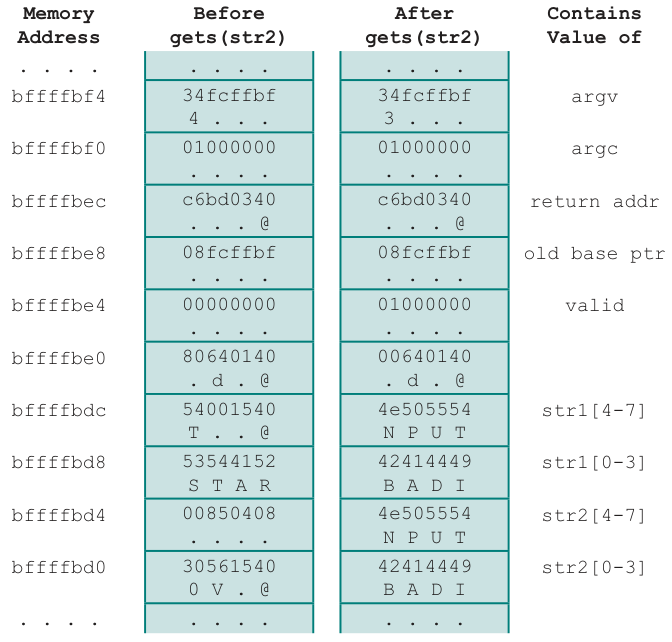
\includegraphics[width=\textwidth]{media/t08/desbordamientoPilaMemoria.png}
    \caption{Mecanismo de desbordamiento de búfer en pila con sobreescritura de la dirección de retorno \parencite[\S 15.2, p.\ 664]{stallings2018operating}.}
    \label{fig:desbordamientoPilaMemoria}
\end{figure}

\subsection{Mecanismos y fases de ejecución de ataques}\label{subsec:mecanismosFasesAtaques}

Un \textbf{ataque} (\textit{attack}) se define formalmente como una acción deliberada y planificada ejecutada por un agente hostil para evadir los controles de seguridad, violar las políticas de un sistema y provocar la pérdida de confidencialidad, integridad o disponibilidad de los recursos \parencite[\S 2, p.\ 22]{rfc4949}.

En la ingeniería de seguridad moderna, la progresión temporal de un ataque dirigido se analiza mediante modelos estructurados de ciclo de vida (como la \textit{Cyber Kill Chain} y la matriz MITRE ATT\&CK):
\begin{enumerate}[noitemsep, topsep=2pt]
    \item \textbf{Reconocimiento y exploración (\textit{reconnaissance}):} Fase preliminar donde el atacante mapea la infraestructura mediante técnicas pasivas (análisis de registros de dominio y fuentes públicas OSINT) y activas (escaneo de puertos, barrido de rangos de direcciones IP y detección de versiones de sistemas operativos y demonios en red).
    \item \textbf{Armamento y explotación (\textit{weaponization \& exploitation}):} Desarrollo o adaptación del código de explotación (\textit{exploit}) diseñado para detonar una vulnerabilidad específica detectada en la superficie del objetivo, inyectando la carga útil (\textit{payload}) en el entorno vulnerable \parencite[\S 19.5.4, p.\ 946]{deitel2004operating}.
    \item \textbf{Escalada de privilegios y persistencia:} Una vez obtenido acceso inicial en el sistema operativo, el proceso suele operar en un contexto de usuario restringido. El atacante busca explotar fallos locales en el núcleo o servicios mal configurados para elevar privilegios hacia \textit{root} o \textit{SYSTEM}, estableciendo mecanismos de supervivencia al reinicio del equipo (claves de arranque, servicios ocultos o entradas en el planificador \textit{cron}).
    \item \textbf{Movimiento lateral y exfiltración / impacto:} Desplazamiento del atacante entre distintos nodos de la red interna empleando credenciales recolectadas de la memoria del sistema operativo (por ejemplo, atacando el subsistema LSASS en Windows o volcando tokens de sesión), culminando en la exfiltración masiva de bases de datos o en la detonación de mecanismos destructivos o de cifrado coercitivo.
\end{enumerate}

\subsection{Tipología de intrusos y modelos de intrusión}\label{subsec:tipologiaIntrusosModelosIntrusion}

El agente humano o entidad automatizada responsable de perpetrar un ataque recibe la denominación técnica de \textbf{intruso} (\textit{intruder}). Un intruso se define formalmente como cualquier sujeto que busca acceder o que accede a un computador o a sus recursos protegidos sin autorización previa o en flagrante extralimitación de las facultades que le fueron concedidas \parencite[\S 15.1, p.\ 659]{stallings2018operating}.

En un estudio seminal que sentó las bases de la detección moderna de intrusiones, James P. Anderson identificó tres clases fundamentales de intrusos en sistemas computacionales compartidos \parencite[\S 1, pp.\ 12--13]{anderson1980computer}, modelo formal adoptado y expandido por Stallings:
\begin{itemize}[noitemsep, topsep=2pt]
    \item \textbf{Impostor o suplantador (\textit{masquerader}):} Individuo que carece por completo de autorización para utilizar el sistema y penetra sus controles de acceso explotando la cuenta de un usuario legítimo (mediante sustracción de contraseñas, explotación remota de software o interceptación de tokens). El impostor es predominantemente un atacante externo (\textit{outsider}) \parencite[\S 15.1, p.\ 659]{stallings2018operating}.
    \item \textbf{Infractor o usuario abusivo (\textit{misfeasor}):} Usuario legítimo que dispone de acceso formal al sistema pero accede intencionadamente a programas, datos o recursos para los cuales no posee autorización, o que estando autorizado hace un uso ilícito y desmedido de sus prerrogativas. El infractor es casi invariablemente un atacante interno (\textit{insider}) \parencite[\S 1, p.\ 12]{anderson1980computer}.
    \item \textbf{Usuario clandestino (\textit{clandestine user}):} Individuo que toma el control del modo supervisor del sistema operativo (privilegios de superusuario o administrador) y utiliza este poder irrestricto para suprimir la recolección de eventos, alterar o purgar los registros de bitácora (\textit{logs}) y eludir cualquier mecanismo de auditoría forense posterior. Puede manifestarse tanto desde el interior como desde el exterior \parencite[\S 15.1, p.\ 660]{stallings2018operating}.
\end{itemize}

En los entornos contemporáneos, esta tipología clásica se amplía para abarcar diferentes perfiles motivacionales: actores de amenazas avanzadas persistentes (APT, grupos altamente profesionalizados y financiados por estados con objetivos de ciberespionaje militar o industrial a largo plazo), sindicatos de cibercrimen organizado impulsados por el lucro financiero directo, activistas informáticos (\textit{hacktivistas}) motivados por reivindicaciones ideológicas, y atacantes novatos (\textit{script kiddies}) que ejecutan herramientas y exploits desarrollados por terceros sin comprensión profunda de sus mecanismos de bajo nivel \parencite[\S 19.5.5, p.\ 948]{deitel2004operating}. La Tabla~\ref{tab:comparativaAmenazaVulnerabilidadAtaqueIntruso} resume la interrelación técnica entre estos cuatro conceptos axiales de la seguridad informática.

\begin{table}[htbp]
\centering
\footnotesize
\renewcommand{\arraystretch}{1.1}
\renewcommand{\tabularxcolumn}[1]{m{#1}}
\setlength{\emergencystretch}{1.5em}
\caption{Comparativa técnica de conceptos axiales: amenaza, vulnerabilidad, ataque e intruso.}
\label{tab:comparativaAmenazaVulnerabilidadAtaqueIntruso}
\begin{tabularx}{\textwidth}{>{\centering\arraybackslash}m{2.3cm} X X}
\toprule
\textbf{Entidad} & \textbf{Definición técnica y naturaleza} & \textbf{Manifestación en el sistema operativo y mitigación} \\
\midrule
\textbf{Amenaza} & Agente, circunstancia o evento potencial capaz de causar daño al explotar una vulnerabilidad. & Tráfico pasivo de escucha o ataques activos DoS; mitigación mediante cifrado y segmentación de red. \\
\addlinespace
\textbf{Vulnerabilidad} & Debilidad o fallo intrínseco en diseño, código o configuración que permite eludir controles. & Desbordamiento de pila/montículo y defectos TOCTOU; mitigación con canarios de pila, ASLR y validación. \\
\addlinespace
\textbf{Ataque} & Acción deliberada y planificada que materializa una amenaza sobre una debilidad del sistema. & Inyección de shellcode, explotación remota y escalada de privilegios; mitigación con IDS/IPS y EDR. \\
\addlinespace
\textbf{Intruso} & Actor o proceso que intenta acceder o que accede sin autorización formal al sistema. & Suplantador (\textit{masquerader}), infractor (\textit{misfeasor}) y clandestino; mitigación con MFA, PAM y auditoría. \\
\bottomrule
\end{tabularx}
\end{table}

\section{Software malicioso y sus variedades}\label{sec:softwareMaliciosoVariedades}

La explotación de vulnerabilidades en el software y en el sistema operativo alcanza su máxima complejidad técnica mediante el desarrollo de programas hostiles concebidos para alterar el flujo regular de ejecución computacional. El software malicioso o \textit{malware} comprende un ecosistema heterogéneo de artefactos binarios y scripts diseñados para infiltrarse en sistemas de cómputo, eludir las barreras de protección del núcleo y comprometer los activos digitales de organizaciones y usuarios.

\subsection{Definición y taxonomía estructural del malware}\label{subsec:definicionTaxonomiaMalware}

El estándar RFC 4949 define el \textbf{software malicioso} (\textit{malware}) como cualquier programa o fragmento de código introducido encubiertamente en un sistema con la intención deliberada de violar la confidencialidad, comprometer la integridad o menoscabar la disponibilidad de los datos, aplicaciones o recursos del sistema operativo anfitrión \parencite[\S 2, p.\ 183]{rfc4949}. A diferencia de los fallos accidentales de programación, el malware se distingue por una intencionalidad hostil explícita en su diseño algorítmico.

En la arquitectura de sistemas computacionales, Stallings formula una taxonomía ortogonal canónica para clasificar el software malicioso a partir de dos criterios estructurales independientes \parencite[\S 15.1, p.\ 659]{stallings2018operating}:
\begin{enumerate}[noitemsep, topsep=2pt]
    \item \textbf{Criterio de dependencia de programa anfitrión:}
    \begin{itemize}[noitemsep, topsep=1pt]
        \item \textit{Malware parasitario (\textit{parasitic}):} Fragmentos de código que carecen de existencia autónoma y requieren acoplarse físicamente a un archivo ejecutable, programa de utilidad o script legítimo preexistente para ser cargados en memoria por el cargador del sistema operativo. Comprende a los virus informáticos, las bombas lógicas y las puertas traseras insertadas en el código fuente o en binarios.
        \item \textit{Malware independiente (\textit{independent}):} Programas completos y autosuficientes que pueden ser planificados, cargados y ejecutados de forma directa por el núcleo como procesos independientes dentro de la tabla de procesos. Comprende a los gusanos de red y a los agentes zombi o bots.
    \end{itemize}
    \item \textbf{Criterio de replicación:}
    \begin{itemize}[noitemsep, topsep=1pt]
        \item \textit{Malware no replicable:} Artefactos que no generan copias de sí mismos; su ciclo de activación responde exclusivamente a disparadores preconfigurados o instrucciones externas de control (por ejemplo, bombas lógicas y troyanos).
        \item \textit{Malware autorreplicable:} Programas o fragmentos infecciosos que, al ser interpretados o ejecutados por el procesador, generan una o múltiples copias idénticas o mutadas de su propio código para propagarse hacia otros archivos, volúmenes de almacenamiento o nodos interconectados en red (como virus y gusanos).
    \end{itemize}
\end{enumerate}

\subsection{Malware parasitario e infeccioso: virus y bombas lógicas}\label{subsec:malwareParasitarioVirusBombas}

Un \textbf{virus informático} representa el arquetipo del malware parasitario autorreplicable. Su mecanismo operativo requiere infectar programas huéspedes incrustando en ellos una copia de su código malicioso, asegurando que cuando el usuario o el sistema invoque el archivo infectado, el código del virus se ejecute de manera inadvertida \parencite[\S 19.5.2, p.\ 943]{deitel2004operating}. El ciclo de vida de un virus clásico se estructura en cuatro fases cronológicas:
\begin{enumerate}[noitemsep, topsep=2pt]
    \item \textit{Fase latente (\textit{dormant phase}):} El virus permanece inactivo en el almacenamiento o en memoria, a la espera de que se cumpla un evento desencadenante (una fecha de calendario, un conteo de ejecuciones o una señal del sistema).
    \item \textit{Fase de propagación (\textit{propagation phase}):} El virus clona su rutina infecciosa en otros programas ejecutables, sectores de arranque o documentos con macros dentro del sistema de archivos.
    \item \textit{Fase de detonación (\textit{triggering phase}):} Se valida la condición lógica o temporal que activa la rutina hostil programada.
    \item \textit{Fase de ejecución (\textit{execution phase}):} Se despliega la carga maliciosa (\textit{payload}), la cual puede abarcar desde perturbaciones menores en pantalla hasta el formateo de discos o el borrado masivo de estructuras del sistema de archivos.
\end{enumerate}

Según el objetivo y la técnica de acoplamiento en el sistema operativo, los virus se clasifican en:
\begin{itemize}[noitemsep, topsep=2pt]
    \item \textbf{Virus de sector de arranque (\textit{boot sector virus}):} Sobrescriben el registro de arranque maestro (MBR, \textit{master boot record}) o el sector de arranque de la partición activa. Al inicializarse la máquina, la BIOS o firmware transfiere el control al código del virus antes de que el núcleo del sistema operativo cargue sus propios controladores de memoria protegida, otorgándole control irrestricto sobre el hardware \parencite[\S 15.2, p.\ 518]{silberschatz2006fundamentos}.
    \item \textbf{Virus de archivo ejecutable:} Modifican binarios en formatos ejecutables estándar (ELF en Unix/Linux o PE en Windows). Pueden acoplarse al inicio del archivo (\textit{prepending}), al final (\textit{appending}) o en zonas de relleno entre secciones alineadas en disco (\textit{cavity viruses}), alterando el encabezado del ejecutable para desviar el punto de entrada (\textit{Entry Point}) hacia el código viral antes de devolver el flujo al programa legítimo.
    \item \textbf{Macrovirus:} Explotan las capacidades de automatización mediante lenguajes interpretados (como VBA) incrustados en documentos ofimáticos, infectando plantillas globales de la aplicación para replicarse con cada nuevo archivo generado.
    \item \textbf{Mecanismos avanzados de evasión:} Los virus \textit{polimórficos} evaden los motores basados en firmas mediante un motor de cifrado que transmuta la clave y la rutina descifradora en cada infección; los virus \textit{metamórficos} prescinden del cifrado y mutan completamente la estructura de su ensamblador mediante sustitución de instrucciones por secuencias semánticamente equivalentes, inserción de instrucciones nulas (NOP) y reordenamiento de bloques básicos \parencite[\S 19.5.2, p.\ 944]{deitel2004operating}.
\end{itemize}

Por su parte, una \textbf{bomba lógica} (\textit{logic bomb}) es un segmento de código parasitario no replicable incrustado deliberadamente en una aplicación legítima, diseñado para activarse de forma destructiva exclusivamente cuando se satisface una condición lógica predeterminada (por ejemplo, la eliminación de la cuenta de nómina de un desarrollador o una fecha fija en el reloj de tiempo real del sistema).

\subsection{Malware autorreplicable en red: gusanos}\label{subsec:malwareAutorreplicableGusanos}

A diferencia de los virus parasitarios, un \textbf{gusano de red} (\textit{worm}) es un proceso independiente y autónomo que no necesita de un archivo ejecutable anfitrión para existir ni requiere de la intervención humana para propagarse \parencite[\S 15.3.1, p.\ 521]{silberschatz2006fundamentos}. Los gusanos aprovechan las interfaces de red del sistema operativo y los servicios de transporte (TCP/UDP) para escanear activamente rangos de direcciones IP en busca de servidores o demonios que presenten vulnerabilidades de software no mitigadas.

El ciclo operativo de propagación de un gusano abarca tres etapas secuenciales automatizadas:
\begin{enumerate}[noitemsep, topsep=2pt]
    \item \textit{Escaneo y sondeo de red:} Generación algorítmica de listas de direcciones IP (escaneo secuencial, pseudoaleatorio o basado en subredes locales) y sondeo masivo sobre puertos específicos para identificar servicios abiertos.
    \item \textit{Explotación remota y transmisión del vector:} Envío de paquetes especialmente malformados hacia el servicio objetivo para detonar fallos de desbordamiento de memoria o fallas de autenticación, inyectando un cargador mínimo o vector de arranque.
    \item \textit{Descarga y activación autónoma:} El vector transferido invoca llamadas al sistema locales para conectarse a la máquina origen, descargar el binario principal del gusano, registrar su ejecución como un nuevo proceso en el núcleo del sistema receptor y reiniciar el ciclo de propagación hacia nuevos objetivos \parencite[\S 15.3.1, p.\ 522]{silberschatz2006fundamentos}.
\end{enumerate}

El caso paradigmático fundacional en la historia de la computación distribuida fue el \textbf{Gusano Morris} de 1988, el cual infectó miles de estaciones de trabajo UNIX conectadas a Internet en cuestión de horas. Morris combinó de forma coordinada tres vectores técnicos de explotación: 1) un desbordamiento de búfer en la llamada \texttt{gets()} del demonio \texttt{fingerd} para ejecutar \texttt{/bin/sh}; 2) el abuso del comando \texttt{DEBUG} en el servidor de correo \texttt{sendmail} para forzar la compilación remota de código en C; y 3) la explotación de relaciones de confianza no autenticadas en la utilidad \texttt{rsh} mediante el análisis de archivos \texttt{.rhosts} y \texttt{/etc/hosts.equiv} en el sistema de archivos local \parencite[\S 15.3.1, pp.\ 521--522]{silberschatz2006fundamentos}.

\subsection{Software de infiltración y control: troyanos, puertas traseras y rootkits}\label{subsec:softwareInfiltracionTroyanosRootkits}

La persistencia del control hostil sobre un sistema operativo se apoya en componentes especializados de infiltración y ocultación:

Un \textbf{caballo de Troya} (\textit{trojan horse}) es un programa que aparenta cumplir una función útil, benigna o atractiva para el usuario (como un juego, una utilidad de compresión o un visor de documentos), pero que contiene rutinas subrepticias ocultas destinadas a eludir los controles de acceso y ejecutar acciones no autorizadas al amparo de los privilegios del usuario engañado \parencite[\S 15.2.1, p.\ 513]{silberschatz2006fundamentos}. Los troyanos suelen operar como puertas de enlace para instalar software espía, desactivar servicios de defensa o descargar componentes maliciosos adicionales.

Una \textbf{puerta trasera} (\textit{backdoor} o \textit{trapdoor}) constituye un mecanismo secreto de acceso que omite los procedimientos ordinarios de autenticación del sistema operativo \parencite[\S 15.2.2, p.\ 514]{silberschatz2006fundamentos}. Puede ser introducida deliberadamente por un programador desleal en el código fuente, generada automáticamente por un compilador alterado, o implantada por un atacante como un demonio en segundo plano que atiende en un puerto TCP no documentado, facilitando el reingreso continuo sin necesidad de contraseñas.

Los \textbf{rootkits} representan la cúspide tecnológica en la evasión de defensas locales. Su objetivo exclusivo radica en mantener el acceso administrativo permanente y ocultar por completo la presencia de procesos maliciosos, archivos, controladores y conexiones de red frente a las herramientas estándar de monitoreo del sistema operativo (como \texttt{ps}, \texttt{top}, \texttt{ls} o \texttt{netstat}) \parencite[\S 15.1, p.\ 658]{stallings2018operating}. Según el nivel de abstracción y anillo de privilegios en el que operan, se dividen en dos categorías:
\begin{itemize}[noitemsep, topsep=2pt]
    \item \textbf{Rootkits en espacio de usuario (\textit{user-mode rootkits}):} Operan en Ring 3 interceptando las llamadas a las bibliotecas dinámicas compartidas del sistema. En entornos Linux se implementan frecuentemente mediante la variable de entorno \texttt{LD\_PRELOAD} para sobrescribir funciones estándar como \texttt{readdir()} o \texttt{open()}; en Windows recurren a la inyección de código y al enganche de llamadas de la API de Win32 (\textit{API hooking}), filtrando las respuestas entregadas al usuario para omitir las líneas que contienen nombres de archivos o procesos maliciosos.
    \item \textbf{Rootkits en espacio de núcleo (\textit{kernel-mode rootkits}):} Se instalan como módulos dinámicos cargables del núcleo (LKM, \textit{loadable kernel modules}) o controladores de dispositivo en Ring 0. Tienen acceso total a la memoria física y a las estructuras internas del sistema operativo. Estos artefactos interceptan la tabla de despacho de llamadas al sistema (\textit{System Call Table}), manipulan directamente las listas doblemente enlazadas de descriptores de procesos (\texttt{task\_struct} en Linux) para desenganchar el proceso malicioso y volverlo invisible al planificador, y alteran los punteros de manejo de interrupciones, impidiendo que el propio sistema operativo advierta la infección.
\end{itemize}

\subsection{Malware de extorsión y espionaje: ransomware, spyware y botnets}\label{subsec:malwareExtorsionEspionajeRansomware}

El ecosistema contemporáneo del cibercrimen ha transformado el malware en una industria orientada a la monetización coactiva y al espionaje corporativo:

El \textbf{ransomware} es un software malicioso que atenta de forma crítica y directa contra la disponibilidad de los datos. Su modo de operación ejecuta el secuestro del sistema de archivos mediante esquemas de cifrado híbrido de alta velocidad: genera localmente una clave simétrica robusta (típicamente AES-256 o ChaCha20) para cifrar los documentos, bases de datos e imágenes del usuario en disco; acto seguido, sella dicha clave simétrica utilizando una clave pública asimétrica (RSA-2048 o Curve25519) controlada remotamente por los atacantes, borrando los respaldos locales del sistema operativo (como los instantáneos \textit{Shadow Copies} en Windows) y exigiendo un rescate financiero en criptomonedas para suministrar la clave privada de descifrado. Su evolución hacia esquemas de \textit{doble extorsión} combina el cifrado con la exfiltración previa de secretos corporativos bajo amenaza de publicación abierta.

El \textbf{spyware} y los \textbf{registradores de pulsaciones de teclado} (\textit{keyloggers}) representan software de vigilancia subrepticia diseñado para recopilar información confidencial, telemetría de navegación, contraseñas y datos bancarios sin el consentimiento del usuario \parencite[\S 15.2.1, p.\ 514]{silberschatz2006fundamentos}. En el sistema operativo, los keyloggers se implementan mediante controladores de filtro en el subsistema de entrada, ganchos de mensajes globales (como \texttt{SetWindowsHookEx}) o lectura directa de descriptores de eventos en Linux (\texttt{/dev/input/event*}), remitiendo la información sustraída a través de canales encubiertos.

Finalmente, una \textbf{red zombi} o \textbf{botnet} es una infraestructura distribuida compuesta por miles de equipos comprometidos (denominados zombis o bots) controlados remotamente por un operador central (\textit{botmaster}) a través de canales de comando y control (C2, \textit{Command and Control}) basados en protocolos HTTP/HTTPS, IRC o redes punto a punto (P2P) \parencite[\S 19.5.3, p.\ 945]{deitel2004operating}. Las botnets son empleadas como plataformas coordinadas para lanzar ataques masivos de denegación de servicio distribuida (DDoS) que colapsan infraestructuras en red, alquilar capacidad de cómputo para minería clandestina de criptomonedas o distribuir campañas masivas de correo no deseado. La Tabla~\ref{tab:comparativaVariedadesMalware} sintetiza las propiedades técnicas y el comportamiento de las principales variedades de malware analizadas.

\begin{table}[!htbp]
\centering
\scriptsize
\renewcommand{\arraystretch}{1.05}
\renewcommand{\tabularxcolumn}[1]{m{#1}}
\setlength{\emergencystretch}{1.5em}
\caption{Comparativa técnica de variedades de software malicioso y su impacto en el sistema operativo.}
\label{tab:comparativaVariedadesMalware}
\begin{tabularx}{\textwidth}{>{\centering\arraybackslash}m{2.2cm} X X}
\toprule
\textbf{Variedad} & \textbf{Categoría estructural y vector de activación} & \textbf{Impacto en el sistema operativo y mecanismo técnico} \\
\midrule
\textbf{Virus} & Parasitario autorreplicable; ejecución de binarios anfitriones por usuario o sistema. & Infección de ejecutables ELF/PE o MBR; mutación polimórfica y desvío de punto de entrada. \\
\addlinespace
\textbf{Bomba lógica} & Parasitaria no replicable; detonada por condición lógica o temporal en software huésped. & Ejecución destructiva condicionada; alteración encubierta de datos o borrado de estructuras. \\
\addlinespace
\textbf{Gusano} & Independiente autorreplicable; escaneo y explotación remota sin intervención humana. & Agotamiento masivo de ancho de banda y sockets; ejecución como proceso autónomo. \\
\addlinespace
\textbf{Troyano} & Independiente no replicable; engaño al usuario mediante software de apariencia útil. & Despliegue de cargas secundarias subrepticias bajo los privilegios del usuario engañado. \\
\addlinespace
\textbf{Rootkit} & Ocultación avanzada en espacio de usuario (Ring 3) o espacio de núcleo (Ring 0). & Modificación de la \textit{System Call Table} y de listas \texttt{task\_struct} para invisibilizar procesos. \\
\addlinespace
\textbf{Ransomware} & Extorsión por secuestro; cifrado híbrido simétrico/asimétrico masivo de archivos. & Pérdida de disponibilidad en disco mediante AES-256 y eliminación forzada de instantáneas. \\
\addlinespace
\textbf{Spyware} & Vigilancia encubierta; ganchos en subsistemas de entrada y lectura de descriptores. & Interceptación de pulsaciones de teclado, sustracción de credenciales y telemetría oculta. \\
\addlinespace
\textbf{Botnet} & Red zombi independiente; control remoto distribuido mediante canales C2 o P2P. & Ejecución sincronizada de inundaciones en ataques DDoS y retransmisión masiva de tráfico. \\
\bottomrule
\end{tabularx}
\end{table}

\section{Herramientas para la protección de sistemas}\label{sec:herramientasProteccionSistemas}

La seguridad computacional exige desplegar tecnologías de defensa en múltiples estratos, desde el filtrado de red hasta el aislamiento en el espacio del núcleo. Bajo el principio de defensa en profundidad, ninguna salvaguarda individual resulta autosuficiente; la protección robusta combina control perimetral, prevención en el host, mitigaciones en el compilador y criptografía aplicada.

\subsection{Cortafuegos y filtrado de tráfico en capas}\label{subsec:cortafuegosFiltradoTrafico}

Un \textbf{cortafuegos} (\textit{firewall}) regula el flujo bidireccional de paquetes entre redes e interfaces según directivas de seguridad \parencite[\S 19.6.1, p.\ 939]{deitel2004operating}. Se estructura en tres generaciones principales:
\begin{itemize}[noitemsep, topsep=2pt]
    \item \textbf{Filtrado sin estado (\textit{stateless}):} Opera en capas 3 y 4 (OSI). Evalúa cabeceras de paquetes (IP origen/destino, puertos TCP/UDP, banderas) de forma aislada mediante reglas secuenciales, sin retener contexto de transacciones.
    \item \textbf{Inspección con estado (\textit{stateful}):} Rastrea en memoria del núcleo el ciclo de conexiones TCP (SYN, ESTABLISHED, FIN/RST) y asociaciones UDP pseudo-estado \parencite[\S 19.6.1, p.\ 940]{deitel2004operating}, admitiendo el tráfico de retorno legítimo y descartando anomalías.
    \item \textbf{Pasarelas de aplicación y WAF:} Operan en capa 7 con inspección profunda de paquetes (\textit{Deep Packet Inspection}) para validar sintaxis de protocolos (HTTP, DNS, TLS), bloqueando inyecciones y alteraciones invisibles al filtrado de transporte.
\end{itemize}

En los sistemas operativos modernos, el cortafuegos se ejecuta en el núcleo. En Linux, el subsistema \textit{netfilter} brinda ganchos de red operados mediante \texttt{iptables} o \texttt{nftables}, segmentando cadenas (\texttt{INPUT}, \texttt{OUTPUT}, \texttt{FORWARD}) con mínima sobrecarga \parencite[\S 15.7, p.\ 546]{silberschatz2006fundamentos}.

\subsection{Sistemas de detección y prevención de intrusos (IDS/IPS)}\label{subsec:sistemasIdsIps}

Los \textbf{sistemas de detección de intrusos} (IDS, \textit{intrusion detection systems}) monitorizan eventos de red y del host para identificar patrones hostiles o transgresiones a las directivas del sistema \parencite[\S 15.1, p.\ 660]{stallings2018operating}. Se dividen según su ámbito en:
\begin{itemize}[noitemsep, topsep=2pt]
    \item \textbf{IDS basados en host (HIDS):} Auditan bitácoras locales, sumas criptográficas de binarios (AIDE, Tripwire) y llamadas al sistema (\textit{syscalls}) para detectar anomalías operativas en procesos \parencite[\S 15.1, p.\ 661]{stallings2018operating}.
    \item \textbf{IDS basados en red (NIDS):} Inspeccionan tráfico promiscuo en segmentos estratégicos (Snort, Suricata) para correlacionar ataques distribuidos.
\end{itemize}

El motor analítico opera por firmas (\textit{signature-based}), de alta precisión contra patrones conocidos pero ineficaz ante ataques de día cero (\textit{zero-day}), o por anomalías (\textit{anomaly-based}), contrastando la actividad frente a perfiles estadísticos de normalidad. Cuando el sistema descarta paquetes o finaliza procesos de forma autónoma, opera como \textbf{sistema de prevención de intrusos} (IPS, \textit{intrusion prevention system}).

\subsection{Motores antimalware y detección en puntos terminales (EDR)}\label{subsec:motoresAntimalwareEdr}

El software antimalware intercepta la ejecución de código malicioso \parencite[\S 19.6.3, p.\ 941]{deitel2004operating} mediante tres métodos: contrastación de huellas criptográficas SHA-256 en repositorios, análisis heurístico de secuencias en ensamblador y confinamiento dinámico en entornos virtuales aislados (\textit{sandboxing}).

En entornos empresariales, estas herramientas han evolucionado a plataformas EDR (\textit{Endpoint Detection and Response}), las cuales capturan telemetría del núcleo a bajo nivel (árboles de procesos, inyecciones de memoria, claves de registro y sockets). Mediante correlación en tiempo real y aprendizaje automático, los EDR aíslan nodos vulnerados y facilitan la contención forense.

\subsection{Mecanismos de aislamiento y endurecimiento del núcleo}\label{subsec:aislamientoEndurecimientoNucleo}

El núcleo del sistema operativo provee mitigaciones estructurales contra vulnerabilidades de memoria y abusos de privilegios \parencite[\S 15.5, p.\ 683]{stallings2018operating}:
\begin{itemize}[noitemsep, topsep=2pt]
    \item \textbf{Aleatorización de memoria (ASLR):} Modifica dinámicamente la dirección base de pila, montículo y bibliotecas, frustrando saltos predecibles en exploits.
    \item \textbf{Prevención de ejecución de datos (DEP / NX bit):} Marca regiones de memoria como no ejecutables ($W \oplus X$) mediante paginación por hardware, impidiendo ejecutar \textit{shellcodes} en búferes.
    \item \textbf{Canarios de pila (\textit{Stack Canaries}):} Valores de guardia insertados por el compilador (\texttt{-fstack-protector}); ante una sobreescritura, \texttt{\_\_stack\_chk\_fail()} termina el proceso de inmediato.
    \item \textbf{Módulos de seguridad obligatoria (LSM):} Extensiones del núcleo como SELinux y AppArmor que confinan procesos bajo reglas de tipo (MAC), neutralizando la escalada aun si se compromete una cuenta administrativa.
    \item \textbf{Aislamiento por contenedores y \textit{seccomp}:} Espacios de nombres (\textit{namespaces}) y grupos de control (\textit{cgroups}) en Linux, combinados con \textit{seccomp-bpf} para restringir las llamadas al sistema permitidas a cada hilo.
\end{itemize}

\subsection{Cifrado de almacenamiento y comunicaciones del sistema}\label{subsec:cifradoAlmacenamientoComunicaciones}

La criptografía salvaguarda la confidencialidad e integridad de la información en reposo y en tránsito:
\begin{itemize}[noitemsep, topsep=2pt]
    \item \textbf{Cifrado en reposo (\textit{data at rest}):} Protege los datos ante sustracción física de discos mediante cifrado de volumen completo (FDE) con LUKS/\texttt{dm-crypt} en Linux o BitLocker en Windows, enlazados al chip TPM del procesador.
    \item \textbf{Cifrado en tránsito (\textit{data in transit}):} Impide la interceptación y alteración por intermediarios mediante TLS 1.3 en capa de aplicación e IPsec en capa de red para enlaces seguros corporativos \parencite[\S 19.10.2, p.\ 960]{deitel2004operating}.
\end{itemize}

\subsection{Herramientas de auditoría y análisis de vulnerabilidades}\label{subsec:auditoriaAnalisisVulnerabilidades}

La postura de seguridad se evalúa continuamente mediante diagnóstico y auditoría forense:
\begin{itemize}[noitemsep, topsep=2pt]
    \item \textbf{Auditoría del núcleo:} El demonio \texttt{auditd} en Linux registra llamadas al sistema, accesos a \texttt{/etc/shadow} y alteraciones de permisos en archivos clave.
    \item \textbf{Escáneres y mapeo de red:} Nmap para prospección de puertos y huellas de servicios; OpenVAS/Greenbone para contrastar versiones contra bases CVE.
    \item \textbf{Auditoría de configuración:} Utilidades como Lynis que evalúan directivas del sistema y cuantifican su índice de endurecimiento.
\end{itemize}

La Tabla~\ref{tab:comparativaHerramientasSeguridad} ofrece una visión comparativa de las principales familias de herramientas de protección analizadas y su ámbito de acción dentro de la infraestructura computacional.

\begin{table}[htbp]
\centering
\footnotesize
\renewcommand{\arraystretch}{1.1}
\renewcommand{\tabularxcolumn}[1]{m{#1}}
\setlength{\emergencystretch}{1.5em}
\caption{Comparativa técnica de herramientas y tecnologías de protección de sistemas.}
\label{tab:comparativaHerramientasSeguridad}
\begin{tabularx}{\textwidth}{>{\centering\arraybackslash}m{2.4cm} X X}
\toprule
\textbf{Categoría} & \textbf{Tecnologías y herramientas representativas} & \textbf{Mecanismo técnico en el sistema e impacto defensivo} \\
\midrule
\textbf{Cortafuegos} & \textit{netfilter} (\texttt{nftables}, \texttt{iptables}), WAF y firewalls con estado. & Inspección dinámica de conexiones en capas 3, 4 y 7; bloqueo de tráfico no autorizado en el núcleo. \\
\addlinespace
\textbf{IDS / IPS} & Snort, Suricata (NIDS/NIPS); OSSEC, Wazuh y Tripwire (HIDS). & Análisis de firmas y detección de anomalías; alerta y descarte activo de paquetes o procesos hostiles. \\
\addlinespace
\textbf{Antimalware / EDR} & Motores antivirus heurísticos, sandboxes virtuales y agentes EDR. & Inspección por firmas SHA-256, telemetría continua de procesos en memoria y aislamiento de nodos. \\
\addlinespace
\textbf{Defensa del núcleo} & ASLR, DEP/NX bit, canarios de pila de GCC, SELinux y AppArmor. & Aleatorización de memoria virtual, páginas no ejecutables ($W \oplus X$) y confinamiento obligatorio MAC. \\
\addlinespace
\textbf{Criptografía} & LUKS con \texttt{dm-crypt}, BitLocker con TPM, TLS 1.3 e IPsec. & Cifrado transparente de volúmenes en reposo y encapsulación segura de tráfico en tránsito en red. \\
\addlinespace
\textbf{Auditoría de SO} & \texttt{auditd}, Nmap, OpenVAS / Greenbone y Lynis. & Registro inmutable de llamadas al sistema, sondeo de servicios expuestos y análisis de fallos CVE. \\
\bottomrule
\end{tabularx}
\end{table}

\section{Recomendaciones para la protección de la información}\label{sec:recomendacionesProteccionInformacion}

La protección efectiva de la información demanda directivas de ingeniería, configuraciones restrictivas en el sistema operativo y procedimientos metodológicos de mantenimiento orientados a reducir la superficie de ataque y garantizar la resiliencia operativa.

\subsection{Principio de mínimo privilegio y defensa en profundidad}\label{subsec:minimoPrivilegioDefensaProfundidad}

La gestión del sistema operativo debe aplicar estrictamente el principio de mínimo privilegio \parencite[\S 14.2, p.\ 484]{silberschatz2006fundamentos}. Los usuarios ordinarios no deben disponer de privilegios de superusuario; las labores administrativas se ejecutan mediante elevación temporal y auditada (\texttt{sudo}). Asimismo, los demonios de red deben confinarse bajo cuentas de servicio sin privilegios mediante perfiles SELinux o AppArmor.

Este esquema se integra con la \textbf{defensa en profundidad} (\textit{defense in depth}), disponiendo controles escalonados (filtrado de red, aislamiento de procesos, permisos estrictos y criptografía) para contener el movimiento lateral ante el compromiso de una capa externa \parencite[\S 19.6, p.\ 939]{deitel2004operating}.

\subsection{Endurecimiento de configuración del sistema operativo}\label{subsec:endurecimientoConfiguracionSo}

El endurecimiento (\textit{hardening}) elimina vectores de riesgo en configuraciones predeterminadas \parencite[\S 15.5, p.\ 681]{stallings2018operating} mediante directivas sistemáticas:
\begin{itemize}[noitemsep, topsep=2pt]
    \item \textbf{Reducción de servicios:} Inhabilitar demonios, compiladores y servicios en red prescindibles (Telnet, FTP, RPC), cerrando puertos no utilizados \parencite[\S 15.5, p.\ 683]{stallings2018operating}.
    \item \textbf{Permisos en archivos:} Fijar máscaras (\textit{umask}) restrictivas (\texttt{027} o \texttt{077}), custodiar \texttt{/etc/shadow}, retirar el bit \textit{SetUID} innecesario y fijar el bit pegajoso (\textit{sticky bit}) en \texttt{/tmp} \parencite[\S 15.5, p.\ 681]{stallings2018operating}.
    \item \textbf{Protocolos cifrados:} Reemplazar transmisiones en texto plano por canales seguros (SSHv2 con claves Ed25519, HTTPS con TLS 1.3 y NTS para tiempo).
\end{itemize}

\subsection{Gestión de parches y mitigación continua de fallos}\label{subsec:gestionParchesMitigacion}

La mitigación de vulnerabilidades lógicas exige una política de gestión de parches (\textit{patch management}) basada en la monitorización de boletines CVE y priorización CVSS \parencite[\S 15.6, p.\ 684]{stallings2018operating}. En servidores de producción, los parches se validan en entornos de prueba previa implementación \parencite[\S 15.5, p.\ 683]{stallings2018operating}, recurriendo a tecnologías de parchado en caliente del núcleo (como Kpatch) para sostener la disponibilidad de servicios ininterrumpidos.

\subsection{Esquemas de respaldo y recuperación ante desastres}\label{subsec:esquemasRespaldoRecuperacion}

Frente al secuestro por ransomware o fallas de hardware, los esquemas de respaldo constituyen la salvaguarda de disponibilidad definitiva. Se aplica la regla 3-2-1: tres copias de los datos en dos medios distintos (disco y almacenamiento externo o nube), manteniendo una copia fuera del sitio.

Para neutralizar la alteración coercitiva, se emplea almacenamiento inmutable WORM o bloqueo de objetos, validando periódicamente las copias mediante simulaciones de restauración para asegurar los objetivos RTO y RPO.

\subsection{Autenticación multifactor y control de identidades}\label{subsec:autenticacionMultifactorIdentidades}

El empleo exclusivo de contraseñas es vulnerable ante ataques de fuerza bruta y suplantación \parencite[\S 19.3.1, p.\ 928]{deitel2004operating}. Se demanda autenticación multifactor (MFA), combinando conocimiento (contraseña), posesión (token TOTP o llave FIDO2) e inherencia (biometría) \parencite[\S 2, p.\ 24]{rfc4949}. En el sistema operativo, estas directivas se imponen mediante módulos PAM, limitación de reintentos y federación con Kerberos.

\subsection{Registro de eventos, monitoreo y respuesta a incidentes}\label{subsec:registroEventosRespuestaIncidentes}

Las bitácoras del sistema deben protegerse contra purgas maliciosas \parencite[\S 15.1, p.\ 660]{stallings2018operating}, reenviando eventos de autenticación, trazas de \texttt{auditd} y del cortafuegos hacia servidores remotos cifrados (syslog vía TLS) y plataformas SIEM.

Asimismo, las entidades deben operar un plan formal de respuesta a incidentes bajo las fases NIST SP 800-61 (preparación, detección, contención, erradicación, recuperación y lecciones aprendidas) \parencite[\S 3, pp.\ 21--43]{nistSp800_61}, garantizando la captura forense de memoria y la restauración ordenada de sistemas.

\section{Conclusiones personales}\label{sec:conclusionesPersonales}

El análisis sistemático desarrollado evidencia que la seguridad informática no constituye un componente accesorio susceptible de añadirse a posteriori sobre un sistema operativo, sino una propiedad arquitectónica emergente que debe concebirse desde el diseño mismo del núcleo y del hardware. La convivencia armónica entre procesos en entornos multiprogramados descansa en el aislamiento provisto por la unidad de administración de memoria, la mediación completa en llamadas al sistema y la separación tajante entre los modos de ejecución de usuario y de supervisor. Cualquier concesión en estos mecanismos estructurales degrada la concurrencia en vector de ataque, pues los modelos formales delimitan con rigor matemático las fronteras de confianza del software.

La disolución irreversible del perímetro defensivo corporativo clásico impone descartar de forma definitiva la presunción de confianza implícita asociada a la topología de red. En el entorno contemporáneo del ciberespacio, donde las amenazas internas y externas convergen mediante el robo de credenciales y el abuso de identidades válidas, el modelo de confianza cero se posiciona como una necesidad técnica insoslayable. Cada interacción entre entidades, cada acceso a descriptores de archivos y cada transferencia de paquetes en el sistema debe autenticarse, autorizarse y cifrarse bajo la premisa operativa de que las barreras perimetrales han sido rebasadas y de que cualquier nodo puede albergar un proceso hostil.

El estudio de las familias de software malicioso revela una confrontación continua entre vectores de explotación y mitigaciones del núcleo. Frente a desbordamientos de memoria en la pila, la ingeniería del sistema operativo integró la aleatorización del espacio de direcciones, la segregación de memoria no ejecutable mediante el bit NX y los canarios de pila. No obstante, el surgimiento de técnicas como la programación orientada al retorno, la mutación polimórfica y la inserción de rootkits en anillos privilegiados demuestra que las salvaguardas reactivas por firmas son insuficientes. El control de acceso obligatorio y el confinamiento de procesos mediante extensiones de seguridad en el núcleo son indispensables para contener de raíz el radio de impacto de vulnerabilidades explotadas.

La fortaleza de una infraestructura computacional radica en su capacidad de resiliencia operativa y contención ante incidentes inevitables, y no en la pretensión utópica de una invulnerabilidad absoluta. La defensa en profundidad, complementada con el endurecimiento del sistema operativo y la gestión proactiva de parches, impide que el compromiso de una capa aislada desencadene una falla sistémica. La protección integral de los activos demanda entrelazar salvaguardas en todos los estratos: cifrado robusto en reposo y tránsito, respaldos inmutables bajo esquemas WORM para neutralizar el ransomware, y auditoría centralizada de eventos para garantizar la trazabilidad forense.

Finalmente, los mecanismos técnicos de protección resultan inoperantes si no se articulan con una disciplina operativa y rigor metodológico en la administración de sistemas. La recurrencia de intrusiones provocadas por configuraciones predeterminadas permisivas o rezagos en actualizaciones evidencia que el factor humano sigue siendo un eslabón determinante en la cadena de seguridad. Para el ingeniero en computación, dominar los fundamentos internos del sistema operativo y los principios formales de la ciberseguridad representa una responsabilidad profesional indeclinable, esencial para salvaguardar la integridad, confidencialidad y continuidad de las infraestructuras que sustentan a la sociedad moderna.

\newpage
\nocite{*}
\printbibliography[heading=bibintoc, title={Referencias}]

\end{document}
